\documentclass[journal]{IEEEtran}
\usepackage{amsmath,amssymb,amsfonts}
\usepackage{amsthm}
\usepackage{graphicx}
\usepackage{booktabs,multirow}
\usepackage{cite}
\usepackage{algorithm}
\usepackage{algorithmic}
\usepackage{url}
\newtheorem{proposition}{Proposition}
\newtheorem{theorem}{Theorem}
\newcommand{\FullOnTimePercent}{98.11\%}
\newcommand{\FullOnTimeCILowPercent}{97.94\%}
\newcommand{\FullOnTimeCIHighPercent}{98.26\%}
\newcommand{\InnovationOneCrossGainPP}{0.05}
\newcommand{\InnovationOneCrossCILowPP}{0.01}
\newcommand{\InnovationOneCrossCIHighPP}{0.08}
\newcommand{\InnovationOneAcceptanceGainPP}{0.12}
\newcommand{\InnovationOneAcceptanceCILowPP}{0.07}
\newcommand{\InnovationOneAcceptanceCIHighPP}{0.16}
\newcommand{\InnovationTwoGainPP}{8.69}
\newcommand{\InnovationTwoCILowPP}{8.37}
\newcommand{\InnovationTwoCIHighPP}{9.01}
\newcommand{\StrongBaselineGainPP}{0.19}
\newcommand{\StrongBaselineCILowPP}{0.13}
\newcommand{\StrongBaselineCIHighPP}{0.26}
\newcommand{\FullRuntimeP95Ms}{40.93}
\newcommand{\ExactOptimalPercent}{100.00\%}
\newcommand{\ExactMeanCompletionGap}{0.000}
\newcommand{\SICViolationCount}{0}
\newcommand{\ConfirmatorySeedCount}{50}


\begin{document}
\title{Interference-Externality-Aware Cross-UAV Pairing and Deadline-Driven Resource Allocation for Full-Reuse NOMA-MEC Networks}
\author{Mingxi~Guan}
\maketitle

\begin{abstract}
Full-frequency-reuse multi-UAV NOMA-MEC systems couple user association and pairing through
cross-UAV interference while sharing finite edge CPU under per-task deadlines. We first develop
an interference-externality-aware scheduler whose Replace, Position, and CrossUAV neighborhoods
recompute the actual serving channel, hard SIC feasibility, cross-UAV interference, and per-UAV
MEC load under a deterministic global first-improvement rule. We then derive the minimum offload
ratio and minimum MEC frequency required by each deadline and use their ordered prefix to maximize
the number of completed tasks under each UAV CPU budget. A unified simulator counts every arriving
task once and evaluates all methods on identical immutable traces. Across \ConfirmatorySeedCount{}
unseen seeds, the full method reaches \FullOnTimePercent{} on-time completion; the isolated
cross-UAV and deadline-allocation contributions are \InnovationOneCrossGainPP{} and
\InnovationTwoGainPP{} percentage points, respectively. The final schedules contain
\SICViolationCount{} SIC violations, and the measured $N=20$ scheduling P95 is
\FullRuntimePNinetyFiveMs{} ms.
\end{abstract}

\begin{IEEEkeywords}
Mobile edge computing, multi-UAV, NOMA, interference externality, user pairing, deadline.
\end{IEEEkeywords}

\section{Introduction}
Mobile edge computing (MEC) brings computation close to resource-limited devices, but radio and
CPU decisions remain coupled by latency constraints~\cite{mao2017survey}. UAV-mounted MEC servers
add flexible coverage at the cost of geometry-dependent channels and coordination
overhead~\cite{zeng2016uav,alhourani2014optimal}. Grouped uplink NOMA improves spectrum reuse by
placing at most two users on a subcarrier and decoding them with successive interference
cancellation (SIC)~\cite{ding2017survey,ali2016dynamic}. When multiple UAVs reuse every
subcarrier, however, moving one task changes both its serving channel and the interference seen
by other UAVs. A per-UAV pairing decision therefore has a network externality.

This work targets a professional engineering question: how can a centralized controller produce
feasible schedules within one slot while maximizing the number of tasks completed before their
deadlines? We make two contributions. First, we introduce an interference-externality-aware
cross-UAV association and pairing search with explicit schedule semantics and a network-level
acceptance rule. Second, we derive deadline-oriented offloading and MEC CPU requirements and prove
that their ordered prefix maximizes admitted-task cardinality for each UAV. The two mechanisms are
ablated independently. We claim neither general global optimality nor a complexity-class result.

\section{Related Work}
UAV communication studies establish the altitude, coverage, and delay tradeoffs that motivate
aerial access~\cite{zeng2016uav,alhourani2014optimal}; UAV-enabled OFDMA work further demonstrates
joint radio scheduling under delay constraints~\cite{wu2018joint}. NOMA surveys and MEC analyses
show that user grouping materially affects uplink rates and computation offloading
performance~\cite{ding2017survey,ding2019impact}. Dynamic clustering and swap-based subchannel
assignment address intra-cell grouping~\cite{ali2016dynamic,di2017sub}, while matching theory
provides useful distributed abstractions~\cite{bayat2016matching}. Bilateral stability need not
imply network efficiency when a match changes third-party utilities
~\cite{sasaki1996two,pycia2012stability}. Our first contribution operationalizes that observation
for full-reuse multi-UAV NOMA-MEC by reevaluating the complete network after every candidate move.

Deadline-aware MEC allocation is commonly formulated as a joint continuous/discrete resource
problem~\cite{mao2017survey,zhu2022multi}. Our second contribution focuses on the maximum number of
deadline-feasible tasks under a hard per-UAV CPU budget. It does not optimize energy, UAV
trajectory, transmit power, or long-horizon queues.

\section{System Model and Problem Formulation}
Consider $K$ fixed-altitude UAVs, $S$ reusable uplink subcarriers, and the task set
$\mathcal A_t$ arriving in slot $t$. Task $i$ is represented once by
$(D_i,C_i,T_i,f_i^{\mathrm{loc}})$: input bits, required cycles, relative deadline, and local CPU.
A schedule entry $(i,k,s,r)$ records the actual serving UAV, subcarrier, and NOMA role
$r\in\{\mathrm{strong},\mathrm{weak},\mathrm{solo}\}$. A task appears in at most one entry and a
UAV--subcarrier block contains at most two tasks.

Let $h_{i,k}$ denote the channel power gain and $p_i$ the transmit power. For task $i$ served by
UAV $k$ on subcarrier $s$, cross-UAV interference is
\begin{equation}
 I_{i,k,s}^{\mathrm{cross}}=\sum_{k'\ne k}\sum_{j\in\mathcal G_{k',s}}p_jh_{j,k}.
\end{equation}
For a strong/weak pair $(a,b)$ ordered at the actual receiver so that
$p_ah_{a,k}\ge p_bh_{b,k}$, the evaluated SINRs are
\begin{align}
 \gamma_a&=\frac{p_ah_{a,k}}{p_bh_{b,k}+I_{k,s}^{\mathrm{cross}}+\sigma_s^2},\\
 \gamma_b&=\frac{p_bh_{b,k}}{\epsilon p_ah_{a,k}+I_{k,s}^{\mathrm{cross}}+\sigma_s^2}.
\end{align}
The pair is feasible only if $\gamma_a\ge\Gamma_{\mathrm{SIC}}$; this is a hard system
constraint, not a Shannon-capacity lower bound. Rates are $R_i=B_s\log_2(1+\gamma_i)$.

With offload ratio $\alpha_i$ and MEC allocation $f_i$, completion delay is
\begin{equation}
 L_i=\max\left\{\frac{(1-\alpha_i)C_i}{f_i^{\mathrm{loc}}},
 \frac{\alpha_i(1+\rho)D_i}{R_i}+\frac{\alpha_iC_i}{f_i}\right\}.
\end{equation}
The primary objective is the number of tasks with $L_i\le T_i$. Deterministic tie breakers maximize
total slack and then minimize cross-UAV interference. Every UAV satisfies
$\sum_i f_i\le F_k$.

\section{Interference-Externality-Aware Association and Pairing}
The initializer enumerates feasible solo and two-user groups on each UAV and solves a small binary
linear program subject to task uniqueness and $S$ block slots. If numerical SIC evaluation rejects
a selected pair, the weak member is removed and the strong member remains as a solo transmission.

The local search scans three canonical neighborhoods. \emph{Replace} substitutes an unscheduled
task into a block on its nearest UAV. \emph{Position} swaps users across subcarriers of one UAV.
\emph{CrossUAV} swaps users between blocks on different UAVs, changing their actual serving UAVs.
After role normalization, every candidate is evaluated from scratch using its actual receiver,
cross interference, hard SIC, and per-UAV CPU allocation. A candidate is accepted only if its
network lexicographic objective strictly improves; the scan then restarts in stable-key order.

\begin{proposition}
With a finite task set, finite UAV--subcarrier blocks, and strict lexicographic improvement, the
search terminates after finitely many accepted schedules.
\end{proposition}
\begin{proof}
The structural constraints induce a finite set of schedules. Strict improvement prevents revisiting
an accepted objective/schedule state, and an explicit visited set rejects repeated candidates.
Hence the accepted sequence is finite. The result is neighborhood-local, not globally optimal.
\end{proof}

\section{Deadline-Driven Offloading and MEC Allocation}
The smallest offload fraction that makes the local branch meet the deadline is
\begin{equation}
 \alpha_i^{\min}=\max\!\left(0,1-\frac{T_i f_i^{\mathrm{loc}}}{C_i}\right).
\end{equation}
For $\alpha_i^{\min}>0$, the minimum MEC frequency is
\begin{equation}
 f_i^{\min}=\frac{\alpha_i^{\min}C_i}
 {T_i-\alpha_i^{\min}(1+\rho)D_i/R_i}.
\end{equation}
A non-positive denominator makes the radio link deadline-infeasible. Local-feasible tasks consume
zero MEC CPU. Remaining feasible tasks are ordered by $(f_i^{\min},i)$ and the longest prefix that
fits $F_k$ is admitted.

\begin{theorem}
The nondecreasing-$f_i^{\min}$ prefix maximizes the number of admitted tasks under one UAV CPU
budget when each admitted task yields unit completion value.
\end{theorem}
\begin{proof}
For any feasible set of $m$ tasks, replacing a selected task by an unselected task with no larger
CPU requirement cannot increase total CPU. Repeated exchanges transform it into the $m$ smallest
requirements. Therefore, if that prefix exceeds the budget, no $m$-task set is feasible; the
largest feasible prefix has maximum cardinality.
\end{proof}

\section{Implementation and Experimental Protocol}
The simulator generates an immutable trace per seed. All methods receive identical task IDs,
arrivals, true channels, and estimated channels; the evaluator counts every arrival exactly once.
The frozen confirmatory set contains \ConfirmatorySeedCount{} seeds with $N=20$, $K=2$, $S=3$,
100 slots, a 5 MHz channel, and 4 GHz CPU per UAV. Baselines include local-only, greedy,
interference-aware greedy, per-UAV ILP, exchange-stable matching, intra-UAV global search, and a
fair OFDMA scheduler. Pairing uses a strict $2\times2$ topology/acceptance ablation; resource
allocation compares deadline/minimum-CPU against crossing/equal and fixed-half/equal policies.

Same-seed differences use a deterministic percentile bootstrap
~\cite{efron1993bootstrap}, Wilcoxon signed-rank tests~\cite{wilcoxon1945individual}, Holm
family-wise correction~\cite{holm1979simple}, and matched rank-biserial effect size
~\cite{kerby2014simple}. Separate suites vary interference coupling, $N$, $K$, noise figure, CSI
error, SIC residual and threshold, CPU, deadline, and task load. A complete small-instance
enumeration is used only as an empirical reference.

\section{Results and Mechanism Analysis}
The full method reaches \FullOnTimePercent{} with a 95\% bootstrap interval
[\FullOnTimeCILowPercent{}, \FullOnTimeCIHighPercent{}]. Against the predeclared strongest
controlled baseline, exchange-stable matching, the gain is \StrongBaselineGainPP{} percentage
points with interval [\StrongBaselineCILowPP{}, \StrongBaselineCIHighPP{}]. Figure
\ref{fig:main} reports all main baselines.

\begin{figure}[t]
 \centering
 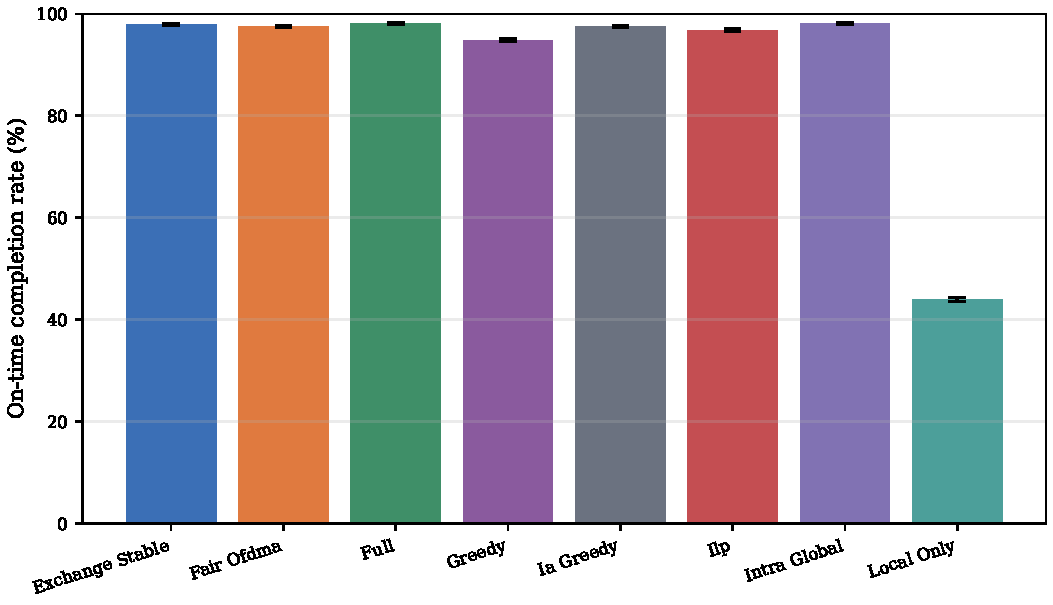
\includegraphics[width=\columnwidth]{../figures/thesis/main_on_time.pdf}
 \caption{Confirmatory on-time completion with deterministic 95\% bootstrap intervals.}
 \label{fig:main}
\end{figure}

The isolated CrossUAV contribution is \InnovationOneCrossGainPP{} percentage points
[\InnovationOneCrossCILowPP{}, \InnovationOneCrossCIHighPP{}], while changing bilateral to global
acceptance with cross-UAV moves contributes \InnovationOneAcceptanceGainPP{} percentage points
[\InnovationOneAcceptanceCILowPP{}, \InnovationOneAcceptanceCIHighPP{}]. These are statistically
stable but small absolute effects in a high-completion regime; Fig.~\ref{fig:pairing} therefore
retains a zero-based axis and the numerical intervals carry the inferential claim.

\begin{figure}[t]
 \centering
 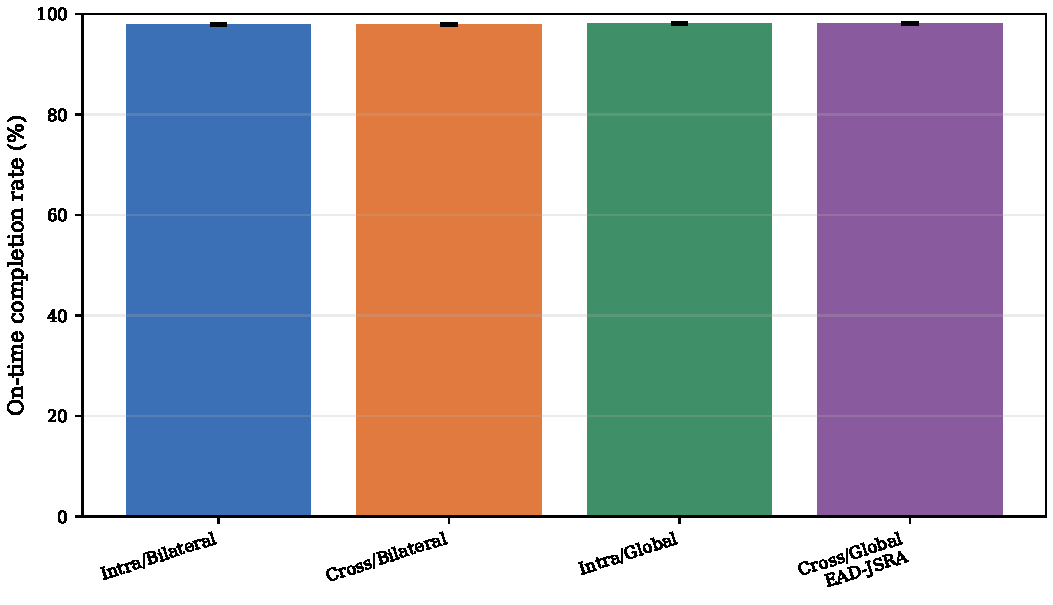
\includegraphics[width=\columnwidth]{../figures/thesis/pairing_ablation.pdf}
 \caption{Pairing topology and acceptance-rule ablation.}
 \label{fig:pairing}
\end{figure}

Deadline/minimum-CPU allocation improves over crossing/equal by \InnovationTwoGainPP{} percentage
points [\InnovationTwoCILowPP{}, \InnovationTwoCIHighPP{}], a materially larger engineering effect
(Fig.~\ref{fig:resource}). The complete small-instance enumeration is matched in
\ExactOptimalPercent{} of slots with mean completion-count gap \ExactMeanCompletionGap{}; this is
not a general optimality guarantee. Across evaluated final schedules, the recorded SIC violation
count is \SICViolationCount{}. The measured $N=20$ scheduling P95 is
\FullRuntimePNinetyFiveMs{} ms.

\begin{figure}[t]
 \centering
 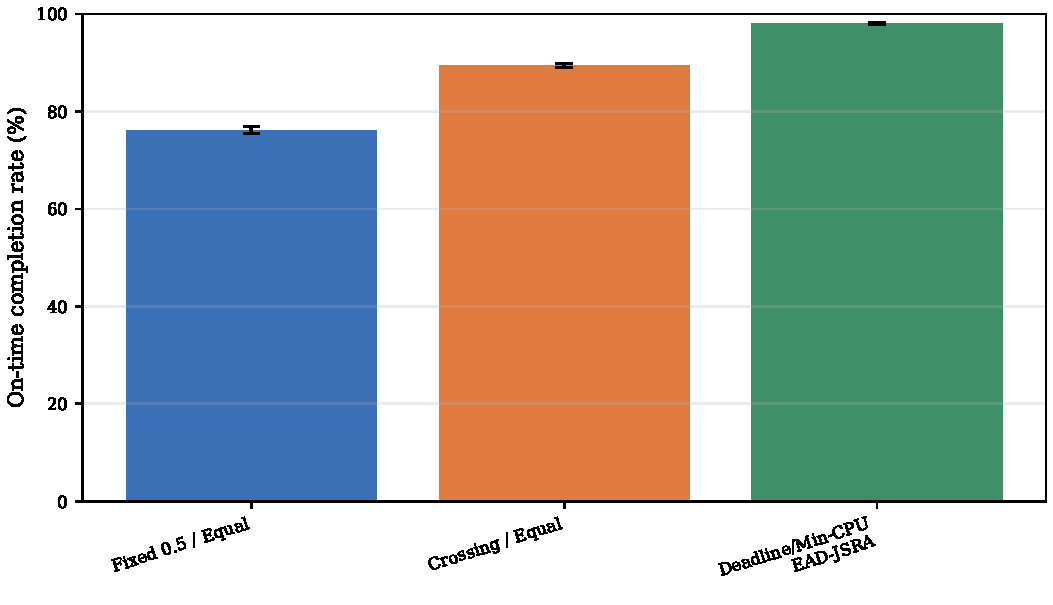
\includegraphics[width=\columnwidth]{../figures/thesis/resource_ablation.pdf}
 \caption{Deadline-oriented resource-allocation ablation.}
 \label{fig:resource}
\end{figure}

\begin{table*}[t]
\centering
\caption{Paired confirmatory comparisons and main engineering metrics.}
\begin{tabular}{lrrrr}
\toprule
Comparison & $\Delta$ (pp) & 95\% CI & $p_{\mathrm{Holm}}$ & $r_{rb}$ \\
\midrule
baseline\_exchange & 0.19 & [0.13, 0.26] & $<0.0001$ & 0.869 \\
baseline\_greedy & 3.24 & [2.96, 3.52] & $<0.0001$ & 1.000 \\
baseline\_ia\_greedy & 0.49 & [0.40, 0.59] & $<0.0001$ & 0.984 \\
baseline\_ilp & 1.30 & [1.16, 1.43] & $<0.0001$ & 1.000 \\
baseline\_ofdma & 0.58 & [0.45, 0.72] & $<0.0001$ & 0.950 \\
innovation1\_acceptance & 0.12 & [0.07, 0.16] & 0.0004 & 0.709 \\
innovation1\_cross & 0.05 & [0.01, 0.08] & 0.0201 & 0.521 \\
innovation2\_deadline & 8.69 & [8.37, 9.01] & $<0.0001$ & 1.000 \\
resource\_fixed\_half & 21.97 & [21.36, 22.60] & $<0.0001$ & 1.000 \\
\bottomrule
\end{tabular}

\bigskip

\begin{tabular}{lrrrrrr}
\toprule
Method & On-time (\%) & Drop (\%) & Delay (s) & Jain & CPU (\%) & P95 (ms) \\
\midrule
exchange\_stable & 97.91 & 2.09 & 0.6841 & 0.9993 & 33.58 & 30.14 \\
fair\_ofdma & 97.52 & 2.48 & 0.6837 & 0.9986 & 31.61 & 0.63 \\
full & 98.11 & 1.89 & 0.6843 & 0.9994 & 34.33 & 40.93 \\
greedy & 94.86 & 5.14 & 0.6804 & 0.9937 & 32.41 & 0.82 \\
ia\_greedy & 97.61 & 2.39 & 0.6838 & 0.9991 & 36.61 & 10.40 \\
ilp & 96.81 & 3.19 & 0.6828 & 0.9984 & 32.20 & 24.26 \\
intra\_global & 98.06 & 1.94 & 0.6843 & 0.9994 & 33.88 & 32.53 \\
local\_only & 43.94 & 56.06 & 0.5417 & 0.9707 & 0.00 & 0.19 \\
\bottomrule
\end{tabular}

\end{table*}

\begin{table}[t]
\centering
\caption{Robustness cases from canonical evidence.}
\resizebox{\columnwidth}{!}{\begin{tabular}{lrr}
\toprule
Case & Exchange-Stable (\%) & EAD-JSRA (Proposed) (\%) \\
\midrule
cpu2 & 90.93 & 91.48 \\
cpu4 & 97.91 & 98.11 \\
cpu8 & 98.92 & 99.04 \\
csi0 & 97.91 & 98.11 \\
csi05 & 97.75 & 97.93 \\
csi10 & 97.63 & 97.68 \\
csi20 & 97.33 & 97.43 \\
eps0 & 98.27 & 98.44 \\
eps02 & 97.91 & 98.11 \\
eps05 & 97.67 & 97.86 \\
eps10 & 97.43 & 97.64 \\
load\_default & 97.91 & 98.11 \\
load\_heavy & 47.67 & 48.04 \\
load\_light & 100.00 & 100.00 \\
nf10 & 97.89 & 98.09 \\
nf3 & 97.94 & 98.12 \\
nf7 & 97.91 & 98.11 \\
sic0 & 97.91 & 98.11 \\
sic3 & 97.14 & 97.32 \\
sic5 & 95.90 & 96.07 \\
sicm3 & 98.21 & 98.41 \\
t06 & 85.16 & 85.57 \\
t08 & 97.91 & 98.11 \\
t10 & 99.77 & 99.80 \\
\bottomrule
\end{tabular}
}
\end{table}

The interference-control curve shows that all methods degrade as coupling increases, while the full
method remains above exchange-stable at all three declared levels; the gap is not monotone.
Scalability results show degradation with $N$ and saturation as $K$ grows. At $K=1$ the full method
is slightly below exchange-stable, and at $K=5$ they tie, so strict dominance is not claimed outside
the multi-UAV main setting.

\section{Engineering Implications and Limitations}
The implementation is suitable for a centralized slot controller with task metadata, estimated
CSI, UAV synchronization, and a control channel capable of distributing schedules. Coordination
cost grows with candidate evaluations and exchanged CSI. Robustness experiments cover estimation
error and residual SIC, but the simulator does not model channel aging during signaling.

UAV trajectories, transmit powers, battery dynamics, long-horizon queues, and field deployment are
outside the active optimization boundary. Parameters are evaluated through Monte Carlo simulation;
no claim of real-world deployment validation is made. PPO and MAPPO remain historical exploratory
code and are not core baselines because the trusted problem is a deterministic combinatorial
scheduler. Future work should study distributed screening, measured pedestrian traces, and joint
trajectory/power control without changing the two contributions reported here.

\section{Conclusion}
This paper presented two independently ablated mechanisms for full-reuse multi-UAV NOMA-MEC: a
cross-UAV association/pairing search that internalizes interference externalities, and a
deadline-derived offloading/CPU allocator that maximizes admitted-task cardinality per UAV. Frozen
same-seed experiments, hard invariant checks, robustness suites, and complete small-instance
enumeration support the stated scope. The evidence shows a small but reliable first contribution
and a large second contribution, with deployment assumptions and non-dominant edge cases reported
explicitly.

\bibliographystyle{IEEEtran}
\bibliography{refs_v2}
\end{document}
